% THIS IS SIGPROC-SP.TEX - VERSION 3.1
% WORKS WITH V3.2SP OF ACM_PROC_ARTICLE-SP.CLS
% APRIL 2009
%
% It is an example file showing how to use the 'acm_proc_article-sp.cls' V3.2SP
% LaTeX2e document class file for Conference Proceedings submissions.
% ----------------------------------------------------------------------------------------------------------------
% This .tex file (and associated .cls V3.2SP) *DOES NOT* produce:
%       1) The Permission Statement
%       2) The Conference (location) Info information
%       3) The Copyright Line with ACM data
%       4) Page numbering
% ---------------------------------------------------------------------------------------------------------------
% It is an example which *does* use the .bib file (from which the .bbl file
% is produced).
% REMEMBER HOWEVER: After having produced the .bbl file,
% and prior to final submission,
% you need to 'insert'  your .bbl file into your source .tex file so as to provide
% ONE 'self-contained' source file.
%
% Questions regarding SIGS should be sent to
% Adrienne Griscti ---> griscti@acm.org
%
% Questions/suggestions regarding the guidelines, .tex and .cls files, etc. to
% Gerald Murray ---> murray@hq.acm.org
%
% For tracking purposes - this is V3.1SP - APRIL 2009

\documentclass{acm_proc_article-sp}
\usepackage{url}
\begin{document}

\title{ {\ttlit} Stock Market Trend Prediction Using Sentiment Analysis }
\subtitle{Senior Project}

\numberofauthors{1} 
\author{
\alignauthor
Nirdesh Bhandari\titlenote{Student at Earlham College}\\
       \affaddr{Earlham College}\\
       \affaddr{801 National Rd W}\\
       \affaddr{Richmond Indiana}\\
       \email{nbhand14@earlham.edu}
}


\date{25 April 2017}


\maketitle
\begin{abstract}
For decades people have tried to predict the stock markets. Some have used historical price trends to predict future changes, while others rely on their gut feeling to make predictions. The prices of stocks reflect the overall confidence the market has on the stocks. The level of this confidence, according to the behavioral economics, is a collective of society's emotions towards a particular stock, which to some extent influences their decision-making. However, is there a way to know the collective mood of society towards a stock? Can this mood be extracted from newspaper articles and magazines?  To address this question, I turn to the field of Natural Language Processing. With the help of various sentiment dictionaries, I ran various types of sentiment analysis over 1.7million newspaper articles published in The Guardian between 2000 and 2016. I then chart the changing sentiments over a time period against the various stock market indices to see whether or not news sentiment is predictive of economic indicators such as stock prices. 
\end{abstract}


\maketitle
\begin{keywords}
Sentiment Analysis, Stock Market Prediction, Natural Language Processing
\end{keywords}




\section{Introduction}

Predicting the stock market has been a century-old quest promising a pot of gold to those who succeed in it. The difficulty of making these predictions lies in the fact that the stock markets respond to the news. The market confidence a particular stock changes as new developments are made and public opinions shift signaling actions from the investors. Indeed, many previous pieces of research done on the subject have found a correlation between public sentiment and economic indicators.Research done by \cite{asur_predicting_2010} found that public sentiments related to movies as expressed on Twitter could predict box office receipt to a great degree of accuracy. Google search queries have been shown to predict consumer spending and online chat activity affecting book sales. 

Moreover, one prominent study done by \cite{gilbert_widespread_2010} was able to show that the levels of public anxiety correlated with the S&P500 values. Then, one might ask -If public mood and emotions are so indicative of changes in stock prices, why doesn't everyone just use it to get to that pot of gold?  While it is true that collective public sentiment predicts stock values, the larger problem is extracting and quantifying the indicators for these sentiments accurately. One cannot enter into people's minds to know how they feel when they read an article in the newspaper or see a TV segment. Furthermore, different people might react differently to the same news. 

The measure of public opinion can be obtained from many sources. The more prominent sources would be Television, social media, magazines and newspaper while other sources include blogs, reviews, and forums. To review these sources different sentiment tracking techniques can be applied. While it might be easy for a human to read a black of text and understand the meaning behind it, the same task can be very difficult for a machine. The degree of accuracy of a sentiment analysis ultimately depends on how well the classifier can deduce the polarity/sentiment of a sentence. The polarity of a sentence measures whether the meaning conveyed by a sentence is positive or negative and is usually measured on a scale of -1 to 1, where -1 represents a negative sentiment while 1 represents a positive sentiment. Using Textblob \footnote{\url{http://textblob.readthedocs.io/en/dev/}}, a natural language processing package we can evaluate the polarities of sentences. For example, "This fat rat is bigger than a cat" carries a polarity score of 0 while the sentence-" The rat loves cheese more" has a polarity score of 0.5 compared to a -0.7 for "Rat thinks a cat is ugly." While most sentiment analysis tools can easily correctly deduce the polarity of sentences, there are instances where they can fail. Sarcasm, satire, poetry and other complex forms of expressions where the meaning isn't straightforward are some of such instances where even the most complex sentiment analyzers fail. TextBlob returns a 0.83 polarity for the sentence -"You crashed the car? Very good, well done, nice!" However, it is important to note that when dealing with news articles within large corpuses, satire and sarcasm constitute a small share of sentences and their effects are often not significant enough to throw off the polarity aggregates of an entire news section. Before I dive into the details of my program, I will be going over some previous research in the next section. 


\section{Previous Research}


Traditionally sentiments and opinions have been collected using surveys and polls. While these are fairly reliable, they are highly dependent on the sample size. There has always been tremendous potential for research, competitive analysis, and market data collection in being able to recognize human opinion from online documents, chat rooms and news articles. While humans can easily recognize the text in these documents, similar understanding of textual context and common linguistic occurrences proves to be difficult for a machine. 

While most sentiment analysis in the past focused had focused on using statistical approaches to look at adjectives and verbs as well as parts of speech, later work focused on parsing sentences to better understand it. \cite{nasukawa_sentiment_2003} recognized that the essential issue to a sentiment analysis is not only the identification polarity and the strength of that polarity, but it is also important to look at semantic relationships between subjects. Based on the hypothesis that local sentiments affect overall perception more than global sentiments, they used this subject-based approach to achieve a higher accuracy in predicting the overall polarity of a document. Other work done in the field looks at concept-level approaches to sentiment analysis. These methods use a random walk and iterative regression to build a concept-level dictionary. Meanwhile \cite{poria_enhanced_2013} employed an emotion labeling mechanism to sentiment analysis on a concept-level.\cite{takala_gold-standard_2014}

On the other hand, machine learning based sentiment analysis techniques such as Artificial Neural Net (ANN), Random Forest, Support Vector Machines (SVM), Naïve Bayes, Multi-Kernel Gaussian Process (MKGP), XGBoost Regressors(XGB), etc are also used to classify sentiments. However, given the complex nature of linguistic identification, machine-learning approaches rarely attain more than 70\% accuracy \cite{takala_gold-standard_2014}. 

Similar work has been done by \cite{kalyani_stock_2016} where they collected Apple Inc. stock information and news related to Apple Inc. over a time span of three years. They gathered news from Google as well as yahoo finance. Using a sentiment detection algorithm, they collected the sentiments over a preprocessed corpus of news articles. Their sentiment classifier employed a bag of words approach where they counted the number of positive and negative words in each piece. Then using several models of SVM, Random Forest, and Naive Bayes, they obtained an accuracy score range between 75\% to 90\% on the test dataset. Likewise, \cite{kirange_open_nodate} also employed a similar method as done by \cite{kalyani_stock_2016} on Indian stock companies over a ten-year span and got an accuracy score range between 47\% to 75\%.on the test dataset for SVM, KNN and Naive Bayes. They also employed a bag of words approach.



\section{Program Design}


For this project, I decided to build sentiment analysis tool that retrieves, processes, evaluates, visualizes and tests newspaper articles. The goal of my project was to find the correlation between stock prices and the overall market sentiment. Using various sentiment dictionaries to look at overall sentiment of a news article, the program graphs the sentiments over a certain timescale and then compares it to the different stock market indexes. Figure~\ref{fig:software} gives an overall software architecture of my project.The first step involves data collection from using the Guardian API\footnote{\url{http://open-platform.theguardian.com/}}.The second step is to collect data for the stock market indices from Yahoo Finance\footnote{\url{https://finance.yahoo.com/}} for the same time range. The next involves processing the data and creating a workable data frame. Then, the data frame is fed to a sentiment analyzer, which iterates over the articles and returns their sentiment value. The final step involves the visualization of data along with tests for cross-correlation and a simple Random Forrest prediction. As of writing this paper, the source code for my program is hosted on GitHub \footnote{\url{https://github.com/nirdesh1995/CS488_Project} }.

\begin{figure}[htp]
\centering
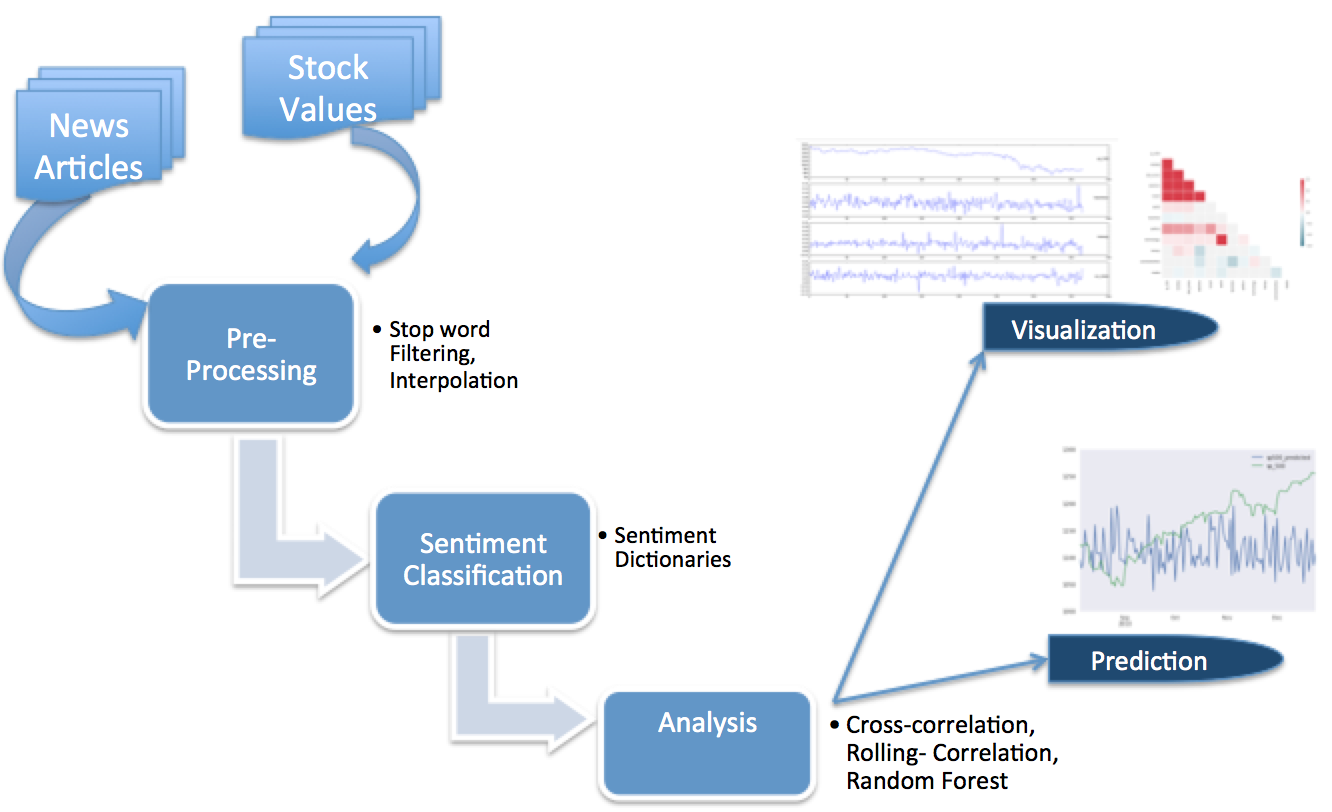
\includegraphics[width=\linewidth,height=6cm]{figures/software_architecture.png}
\caption{Software Architecture}
\label{fig:software}
\end{figure}

\textbf{3.1. Data Collection }


The first task of this project was collecting and compiling a newspaper corpus to run sentiment analysis. While there were corpuses of historical texts and emails available on the Internet, not many online archives provided the articles in a chronological structure with well-organized Metadata. Furthermore, digital forms of newspapers would require text extraction and often had copyright issues. 

I decided to compile my own corpus of news articles. The two helpful APIs I found for this purpose was the NY Times API and The Guardian API. I used the Guardian API to compile a corpus of 1.75 million articles. While the Guardian API was free for developers and offered structure data, it would only return the URL for the articles. So I used python to return daily search queries, open each article and created a compilation of articles of each day. My data was organized on JSON files for each day from the 1st of January of 2000 to 2016. I picked the Guardian API because the data returned contained the Title, date, section ID, web publication date, text publication date and other helpful structured metadata.  

As for the stock data, I decided to use Yahoo Finance and download their historical data for the end of day closing prices for key stock indices to create a pickle file. The Yahoo Finance API also connects to the Pandas\footnote{\url{http://pandas.pydata.org/}} package at python, which makes it convenient for gathering information of various stock prices. For the stock indices, I picked the Standard & Poor's 500, Dow Jones Industrial Average, NASDAQ Composite, Wilshire 5000 Total Market Index and the Russell 2000 Index. I believe that these five indices would be sufficient enough to evaluate various sectors of the economy in respect to what appears on newspaper articles. The program I designed simply takes in the start and the end dates to collect the news articles and stock values.




\begin{figure}[htp]
\centering
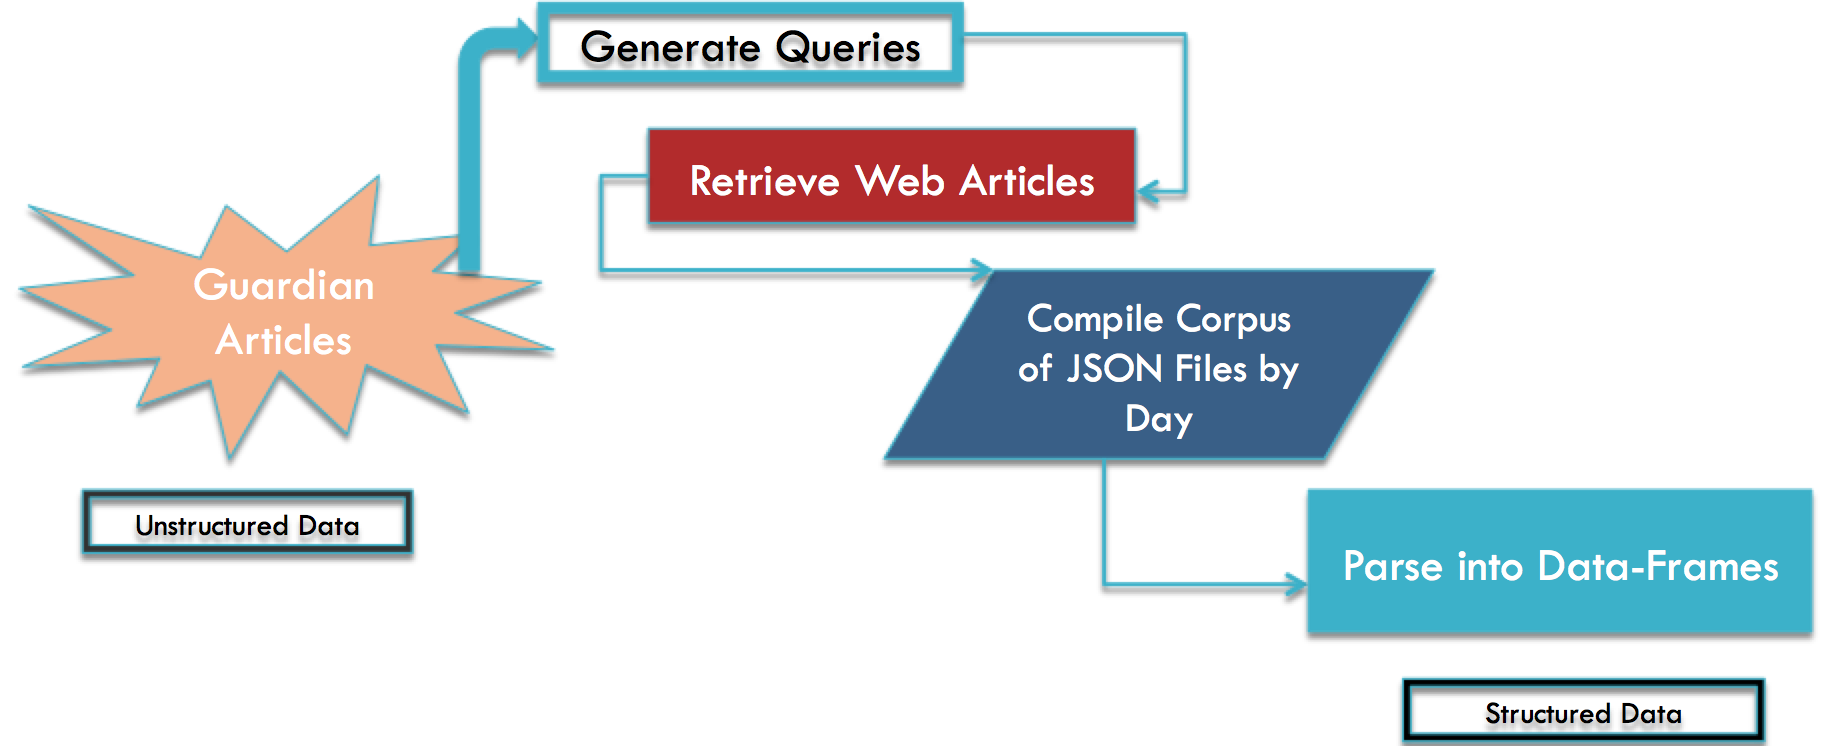
\includegraphics[width=\linewidth, height=5cm]{figures/Data.png}
\caption{Data Collection}
\label{fig:datacoll}
\end{figure}




\textbf{3.2. Pre-Processing }

After creating a corpus of newspaper articles, the next step involved processing the data before it could be fed into the sentiment analyzer. Using the pandas inbuilt JSON package I was able to read and parse articles for a given time period. The JSON files included many unnecessary fields such as weburl, id, pillar-id, etc. Only necessary fields such as publication date, section ID, word count and body-text were used to compile the final data frame. I felt that it would help to save the section ID for the articles as further analysis on different sections (health, money, UK-news, tech, etc.) might improve tests in the future. The process of data collection and processing is shown in  Figure~\ref{fig:datacoll}  

My sentiment analysis was based on evaluating the body text for the articles to receive the sentiment scores. My initial design removed stop words from the body text before compiling the data frame. However, upon a closer inspection of the TextBlob stopwords dictionary, I saw that some of the stop words carried non-neutral polarity scores.  Indeed, as \cite{saif_stopwords_2014} found, removing of stop words to reduce noise from a pre-set dictionary often tends to lower the accuracy of sentiment classification since stop words tend to add contextual information. Therefore, I did not remove stop words from the articles for my analysis. Also, the TextBlob analyzer was not sensitive to upper/lower case and while sentence and word tokenization were initially useful in understanding how the tool worked, it was not relevant later on as I was evaluating entire articles at the same time. 

As for the stock data, I noticed that there were gaps in the time series since stock markets tend to close on weekends and some public holidays. Given the fact that I was dealing with time series data where response lags in variables were expected, I decided to interpolate values for the missing days instead of removing them from my analysis. For this, I used the inbuilt interpolate function of Pandas to evenly space out the values between the gaps. While interpolating with only closing values isn't always the ideal solution, the evenly spaced averaged prices approach is better than not looking at those dates altogether. Since stocks are responsive to news articles and news is published throughout the weekend, my intuition was that not factoring in the weekends altogether would throw off predictions. Furthermore, when data frames for the stocks and polarity values were combined, I noticed that some sections had missing values. The missing values create problems in the visualization and analysis portion later on. Since these missing polarities were occasional, I adopted the simple solution of backfilling the data frame whereby any empty entry would take the value from the next non-empty entry. 


\textbf{3.3. Sentiment Classification}


The two major ways to do a sentiment analysis include either the use of a Lexicon based approach or a Machine-Learning approach. The machine learning approach employs the use of either brute force unsupervised learning or the creation of a classifier using supervised machine learning. The unsupervised approached seemed impractical partly because of the amount of computation it would require and the absence of a proper dataset to train the classifier on. As for the supervised approach, the most common ones included linear neural network classifiers and Naive Bayes and Bayesian Network Probabilistic classifiers. Previous work is done on supervised classifiers often employed a movie review corpus or the use of Amazon reviews to train a classifier. While these approaches were commonly used in previous research, because of the computational complexities and my lack of knowledge in the field, I decided to revisit these later once I had a working model.  Furthermore, my corpus occupied more than 17 gigs of space and training a machine learning classifier for such a large dataset would take an enormous amount of time.

Therefore, I decided to go with a lexicon-based approach for the initial phase. The two popular python packages that I found for this task were Valence Aware Dictionary and sEntiment Reasoner\footnote{\url{https://github.com/cjhutto/vaderSentiment}} (VADER) and TextBlob. Because VADER is designed explicitly for sentiment analysis on social media, I decided to use the TextBlob library. Textblob is built on top of the NLTK package\footnote{\url{http://www.nltk.org/}} in python and seemed to be a reliable tool for classification of news articles. TextBlob employed a lexicon based dictionary approach where a pre-existing dictionary of words, classified based on their polarity values, is used to calculate the overall polarity score of a block of text. TextBlob was particularly useful because of the ease in pre-processing and tokenization as well as sentiment classification. Using text blob, my python tool extracted the sentences out of an article and then use a bag of words approach to return the sentiment polarity scores. The sentiment polarity scores were in the range of -1 to 1, where -1 represented a highly negative article while 1 represented a very positive article. These scores were then aggregated and stored in a Pandas data frame along with the headline of the article, the word count and the sections these articles belonged to. Because of the large size of the corpus, I compiled these polarity value data frames for yearly chunks of news articles. Each year took roughly 20 min to run through the analysis tool.



\textbf{3.4. Visualization  }

Once the polarity scores had complied, the next phase of the project was to take the compilation of these scores and graph them along with the stock prices. Because of how my metadata was organized, I decided to track the aggregate sentiment scores by different sections (for example, health, tech, business, etc.) within the newspaper articles. A quick grouping evaluation showed me that the most of the articles belonged to the following sections: world, business, politics technology, money, and media. While there were other sections such as 'commentisfree', 'film', 'lifeandstyle', etc., these accounted for minimal volume in the corpus. Furthermore, I felt that the film section would not be predictive of changes in the stock market. Because the data spanned 16 years, I decided to look first at chunks of 6-12 months to get a more detailed view of the correlations before scaling it up.

\begin{figure}[htp]
\centering
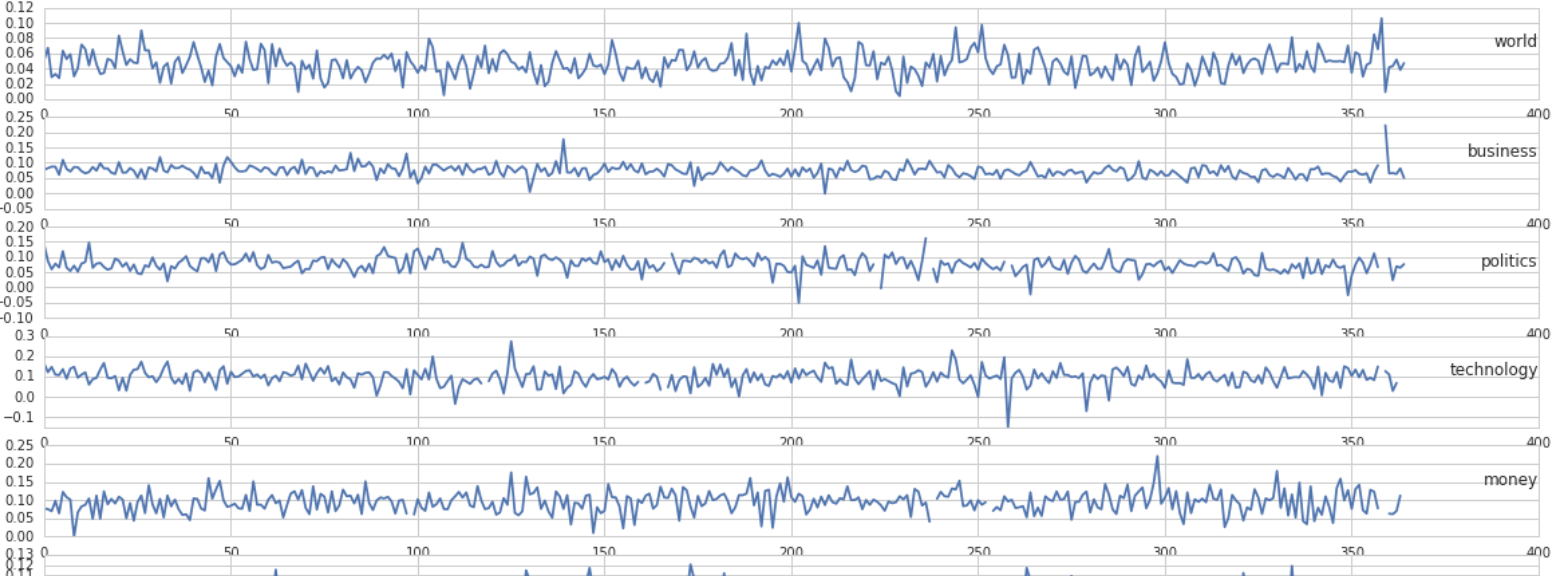
\includegraphics[width=\linewidth, height=5cm]{figures/visual2.png}
\caption{Data Visualization}
\label{fig:datavis}
\end{figure}


The first level of my analysis involved a simple visualization to see how the polarities within these select sections corresponded to the stock prices. Using Matplotlib\footnote{\url{https://matplotlib.org/}}, I was able to graph stock indices along with the polarities. Figure~\ref{fig:datavis} shows an example of the graphs I obtained. 
While the graphs might visually show correlation or the lack of one, it is always more accurate to use a scientific method compare predictability. Therefore, for the second level of analysis, I decided to look at cross-correlations within the stock values and polarities of articles from the different sections. I used the Pandas cross-correlation function for this task. Because I had a total of 11 variables (5 stock indices and 6 section polarities), the cross-correlation table was a 11X11 table with very high correlation values within the stock indices themselves and lower values for correlation between polarities and stocks. Before moving on to other levels of analysis, I decided that visualizing these cross-correlation results would give me a quicker view of the data rather than going over the numbers in a large table. I, therefore, opted for a heat map using the Seaborn\footnote{\url{https://seaborn.pydata.org/}} visualization packet to display the cross-correlation results. Because the correlations I was interested in were the ones between the polarity values and the stock indices, I set a max value of 0.3 for the heat map. This would be helpful to accurately see changes in the smaller correlation values between stocks and polarities since the larger values of stock-stock correlations would simply occupy extreme end of the spectrum. Figure~\ref{fig:corr1} shows one of the heat maps I obtained. 

\begin{figure}[htp]
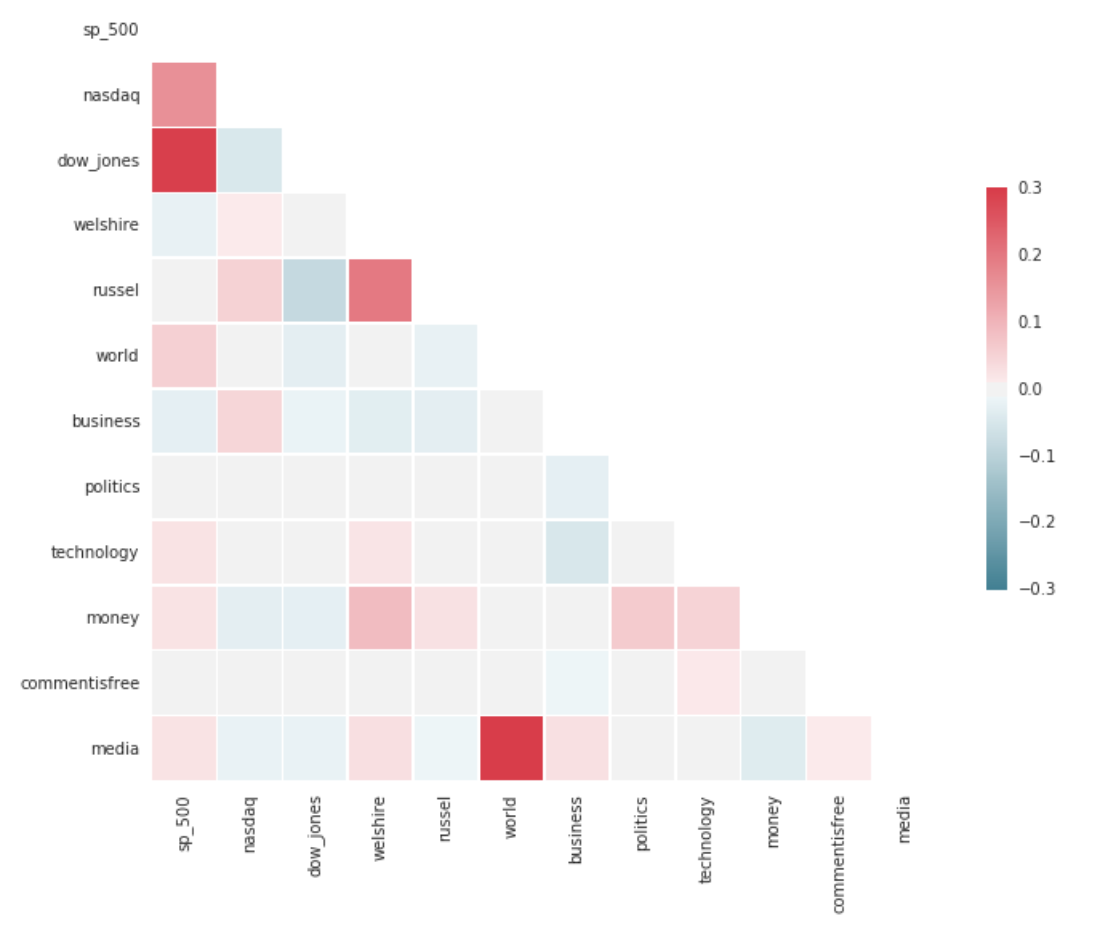
\includegraphics[width=7cm]{figures/heatmap_pct_change.png}
\caption{Correlation Heatmap For Absolute Values}
\label{fig:corr1}
\end{figure}



\textbf{3.5. Analysis }


When looking at the different heat maps, I observed very little correlation between stocks and polarity values. Upon closer examination of the numbers I saw that the stock indices usually consisted of very high values (often in the thousands) while polarity values ranged between -1 and 1. Also, when I looked at polarity numbers of different sections, I realized some sections had a higher average value. This was because news sections consist of a large number of articles and sections like 'technology' would always be predominantly positive. While negative articles would create fluctuations within daily aggregates, the trend line would be higher for some and lower for others. I decided to tackle these problems by evaluating percent changes in daily polarity aggregates and stock-indices. I felt that looking at changes as opposed to absolute values would better improve my analysis. Indeed, looking at percentage changes did show significantly stronger results for cross-correlations and can be seen in Figure~\ref{fig:corr2}. 

\begin{figure}[h]
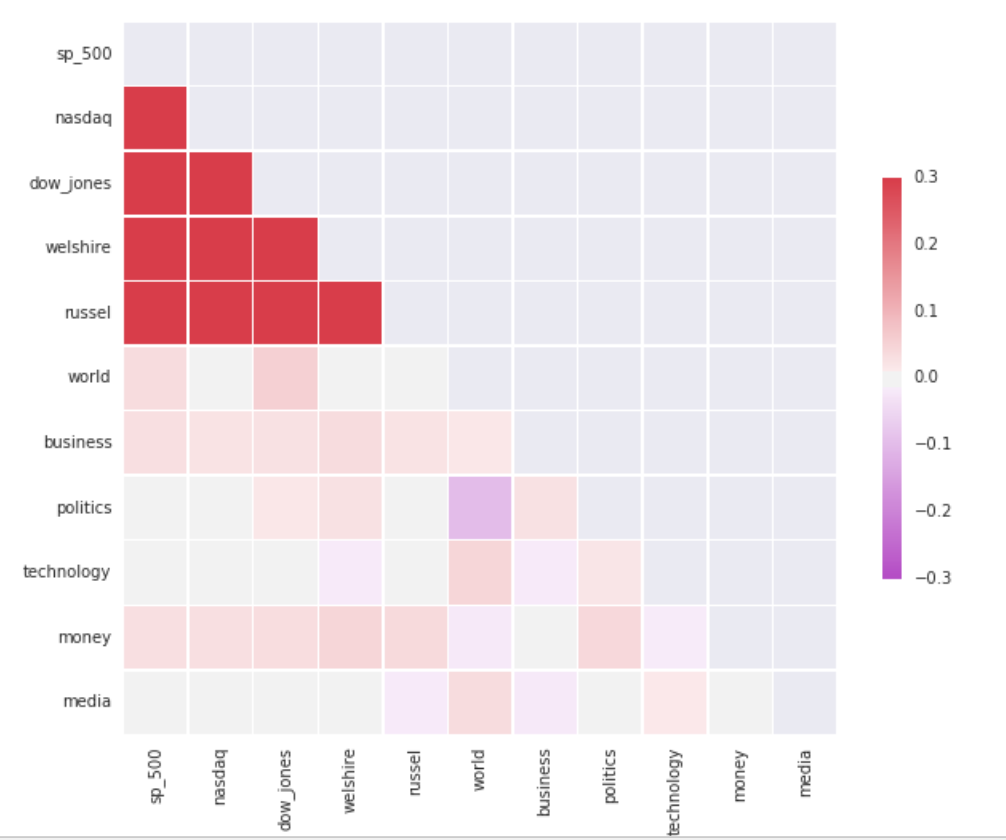
\includegraphics[width=7cm]{figures/improved_corr.png}
\caption{Correlation Heatmap for Percentage Change}
\label{fig:corr2}
\end{figure}

Another factor that I felt would be significant in my analysis was time lag. It often takes time for news to reach people, and response from stock markets could be delayed. Furthermore, I wanted to check if these lags in correlation were different based on the section of the newspaper. Figure~\ref{fig:corrlag} shows the plots for correlations against some sections based on different lag values for S&P500. I found similar graphs when I ran the same tests against NASDAQ prices and Wilshire prices. Figure~\ref{fig:corrlag} shows that the correlation of the 'world' section is slightly higher when the lagged by one day while those for 'business' and 'politics' sections peak at the fourth day. However, given that my data was a time series, the constant peaks and falls over the days led me to believe that this could just be noise within the data. Furthermore, I was also unsure whether the Guardian's publication hours for articles would affect my results. Articles published at 1 am in the morning, as well as articles published at 11:59 pm, are being compiled under the same date while the stock market opens at 9:30 am and closes at 4 pm. However, given the time constraint, I decided to leave that analysis for the future.


\begin{figure}[h]
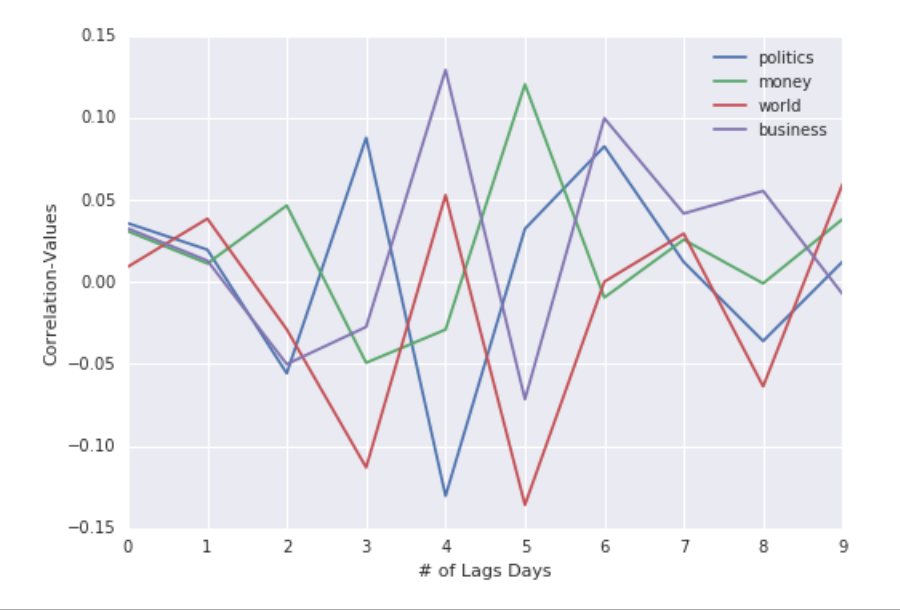
\includegraphics[width=\linewidth]{figures/lag_corr.png}
\caption{Correlation for different lag days}
\label{fig:corrlag}
\end{figure}

\begin{figure}[h]
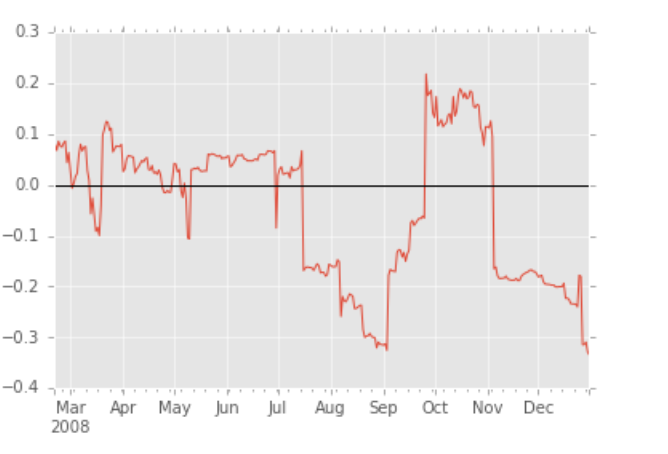
\includegraphics[width=\linewidth]{figures/rolling_corr_money.png}
\caption{Rolling Correlation for Money Section}
\label{fig:rolmoney}
\end{figure}

\begin{figure}[h]
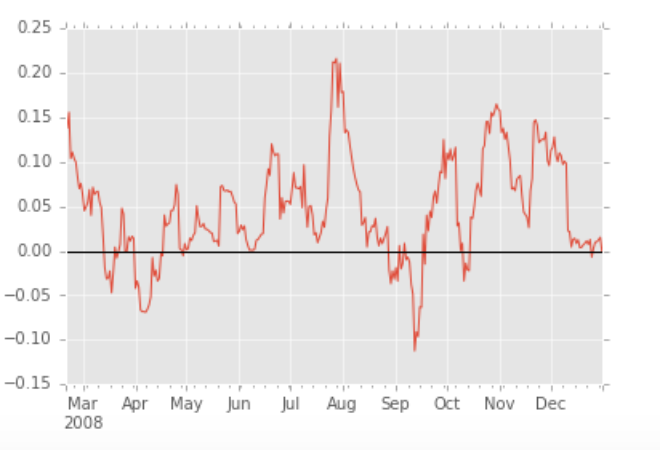
\includegraphics[width=\linewidth]{figures/rolling_corr_tech.png}
\caption{Rolling Correlation For Technology Section}
\label{fig:roltech}
\end{figure}



Likewise, another question I had was whether or not the correlations between sentiments in news articles and stock values changed over time. For example, it would be reasonable to think that during times of financial crises, the news would have more of an impact on stock prices. To test this hypothesis, I decided to use rolling correlation or the dynamic correlation test. In simple terms, a rolling correlation looks at the correlation between two time-series variables as a rolling window calculation. Rolling correlation visualization helps check for changes in correlation over time and can be helpful to detect significant events that shift the relationship of one variable with respect to another \cite{business-science.io_tidy_2017}. I decided to use the rolling correlation between polarity values for money section for the year 2008 and S&P500 prices with a rolling window of 50 days. As Figure~\ref{fig:rolmoney} shows, there were significant shifts in correlation occurring in July and August 2008- right around the time of the Financial Crisis. Meanwhile, when I ran the same test for the 'media' section, the results were different than what was seen with the 'money' section and can be observed in Figure~\ref{fig:roltech}. While finding these significant shifts in themselves might not help predict future price changes in response to the news, the tests confirm that certain sections could be more predictive of stock price movement than others.




\textbf{3.6. Predictive Analytic }


While correlations and visual analysis of polarities within sections of the newspaper and stock indices were useful in getting a closer look at the data, I wanted to predict future prices using these polarities. For this purpose, I tried to implement a simple Random Forest Regression using the Scikit-learn\footnote{\url{http://scikit-learn.org/stable/modules/generated/sklearn.ensemble.RandomForestRegressor.html}} package available for python. For a preliminary experiment, I decided to implement the simplest version of this machine-learning model to produce a predictive graph. Using a training dataset comprised of the first 8 months of 2010, I trained model the to predict S&P500 prices using the polarities of the business, money and world sections. My previous analysis showed that these sections had significantly higher correlation values to S&P500 compared to other sections. Figure~\ref{fig:projection} shows the results I obtained. While my projections were far off from the testing data, I believe that the accuracy of the predictions can be improved using a more extensive training data set and by testing with other models. 

\begin{figure}[h]
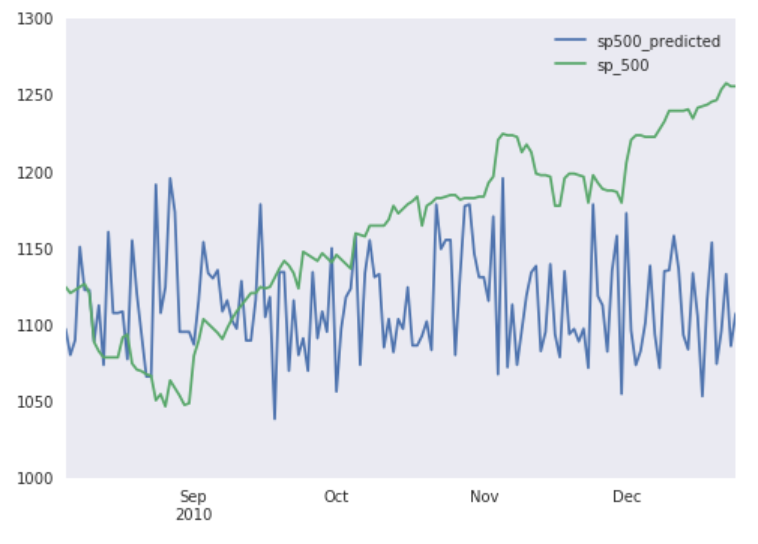
\includegraphics[width=\linewidth]{figures/predictive_model.png}
\caption{Prediction based on Random Forest Regression}
\label{fig:projection}
\end{figure}


\section{Discussion and Future Work}


The field of Natural Language Processing and sentiment analysis for stock predictions turned out to be much larger than I had initially anticipated. Over the course of this project, I realized that there are many different choices of tools at each step and many various methods to analyze and interpret the results. Indeed, if predicting the stocks were that simple, Wall Street would not be investing millions into predictive forecasting programs. Overall I am happy with the work I did for this project. For me, this project was about diving into an unknown field of interest and exploring it best I could within a short timespan. I am sure I could improve my program's prediction capabilities if I keep working on this project in the future. My initial goal for this project was to explore if there was a correlation between sentiments of news articles and stock indices and I was able to meet that goal through this project. There is much I could improve on my statistical tools as well the classifier. During this project I went with the choices that made intuitive sense to me; however, there were many different places where other tools/options could have been employed.

\textbf{4.1. Different Classification Tools}


My project is built on top of a lexicon dictionary-based approach of sentiment classification.  An improvement to this project could be to test the polarities using the various other dictionaries that were initially put aside because of the complexities. This would still be a bag of words method to aggregate sentiment scores. However, certain dictionaries such as the Harvard IV Sentiment Dictionary (HVD) offer as much as 15 categories for sentiments. These dictionaries offer a wider range of sentiment classes and could be helpful to check if other sentiments (besides positive or negative) were more predictive of changes in stock values. Another test could be to use VADER sentiment analysis tool as mentioned above. Furthermore, this pipeline could be implemented in a different set of new articles from the New York Times to check if the sentiments expressed in this century-old newspaper would be more predictive of stock indices.

\textbf{4.2. Other Analytic Methods and Prediction Models}


Further improvements in statistical analysis could be made on this project. One way to see how much a variable affects another is to run a Bivariate Granger Causality Analysis \cite{bollen_twitter_2011}. Simply put, this is a linear regression based econometric test that checks whether changes in values of sentiment scores led to the changes in the value of stocks. Meaning, if the changing sentiment scores in a certain section led to a change in the value of stock, the lagged values on one side show a positive correlation to the effects that took place on the other side. Another method to improve this project would be by using the SOFNN or Self Organizing Fuzzy Neural Network model as described in \cite{bollen_twitter_2011}. Since sentiment trends are not always linearly occurring, this would be a more accurate method to conduct the analysis. However, since SOFNN predicts stock values based on the past n days as an input to self-organize its neurons, and I was dealing with a large dataset. I felt that this would be computationally challenging for this project but would be a great model to check out in the future.

\section{Acknowledgements}
The process of compiling this project has helped me a great deal in polishing my problem solving and analytical skills. The tools that I have acquired over the course of this project will be vital to my possible future career in Data Science. A particular word of gratitude is due to Charlie Peck for guiding my research for this project and for helping me over the course of this semester. 
I would also like to express my most profound appreciation to David Barbella being my Capstone advisor. 



\bibliographystyle{abbrv}
\bibliography{references}

%\balancecolumns 

\end{document}
